\documentclass[11pt]{scrartcl}
\usepackage{dominatrix}

% Graph Drawing Stuff
\usepackage{colortbl}
\usepackage{pgfplots}
\usepackage{tikz}
\usetikzlibrary{trees}
\usetikzlibrary{calc}
\pgfplotsset{compat=1.9}

% Tables
\usepackage{multirow}

% Strikeout
\usepackage{ulem}

% Jon's Name
\newcommand{\jon}{J\'{o}n }

% Additional Definitions
\newcommand{\og}{\ensuremath{\tilde{Y}}}

\title{Monetary Policy}
\subject{ECON W3213 Spring 2014 \jon Steinsson}
\author{Linan Qiu, lq2137}

\begin{document}

\maketitle

\begin{abstract}
This set of recitation notes introduces \textbf{the IS-MP}. This is in no way a substitute for attending lectures, but just in case you dozed off or checked your boyfriend's Facebook page while \jon was working Calculus magic on the board, this set of notes may save you.
\end{abstract}

\section{Derivation}

For the sake of this lesson, the next one, and your undying thirst for knowledge, let's derive the IS-MP diagram.

Investments $I_t$ is

\[I_t = \bar{a}_i \bar{Y}_t - \bar{b}_i \bar{Y}_t (R_t - \bar{r}) \]

Savings $S_t$ is 

\[S_t = Y_t - \bar{a}_s\bar{Y}_t + \bar{b}_s\bar{Y}_t(R_t-r) \]

If you don't know how either of these are derived, check the recitation notes or the lectures notes. It's really straightforward.

Combining these two (hence equating investment and savings) we get

\[\og_t = \bar{a} - \bar{b} (R_t - \bar{r}) \]

This is the \color{blue}IS \color{black} curve.

\begin{figure}[H]
\centering
\begin{tikzpicture}
\begin{axis}[xlabel={Output Gap $\og$},ylabel={Real Interest Rate $R_t$},ymin=0,ymax=10,xmin=0,xmax=10,scale=1,yticklabels={,,}, xticklabels={,,}]
\addplot[blue, domain=0:10]
{-x+8};
\end{axis}
\end{tikzpicture}
\caption{\color{blue}IS Curve}
\end{figure}

It is decreasing in real interest rate $R_t$

\section{Money Demand and Supply}

Now we go back to nominal interest rates. We first argue that the government can change nominal interest rates, then draw the link between nominal and real interest rates, then say that the government can then change real interest rates. 

First let's derive money demand and supply.

On the demand side (remember the equation that we've always been using?)

\begin{align*}
M^d_t V_t &= P_t Y_t \\ 
\log{M^d_t} + \log{V_t} &= \log{P_t} + \log{Y_t} \\
\log{M^d_t} + \phi i_t + v_t &= \log{P_t} + \log{Y_t}
\end{align*}

Now we say that money velocity $V_t$ is not constant. Instead, $\log{V_t} = \phi i_t + v_t$. We get

\[ \log{M_t} + \phi i_t + v_t = \log{P_t} + \log{Y_t} \] 

All this does is to say that the velocity of money is an increasing function o the nominal interest rate.

The central bank simply sets the money supply. In this case, the central bank can set the money supply to achieve any nominal interest rate.

So we can draw something like this

\begin{figure}[H]
\centering
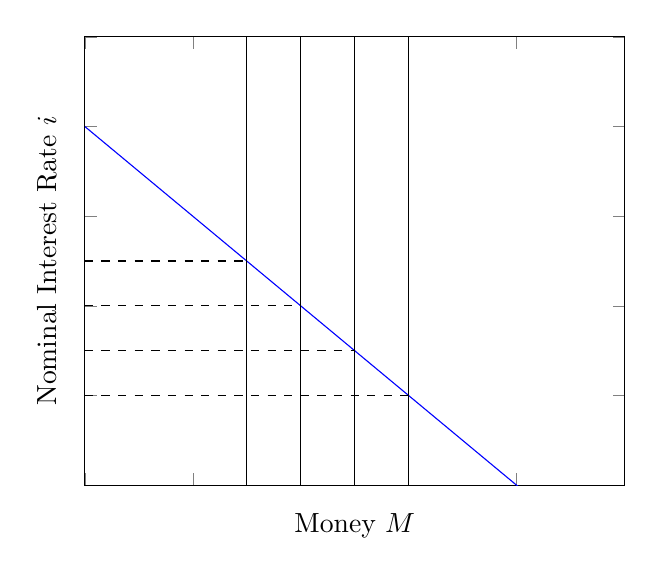
\begin{tikzpicture}
\begin{axis}[xlabel={Money $M$},ylabel={Nominal Interest Rate $i$},ymin=0,ymax=10,xmin=0,xmax=10,scale=1,yticklabels={,,}, xticklabels={,,}]
\addplot[blue, domain=0:10]
{-x+8};
\addplot[black, domain=0:10]
coordinates{(6,0) (6,10)};
\addplot[black, domain=0:10]
coordinates{(5,0) (5,10)};
\addplot[black, domain=0:10]
coordinates{(4,0) (4,10)};
\addplot[black, domain=0:10]
coordinates{(3,0) (3,10)};

\addplot[black, domain=0:10, dashed]
coordinates{(0,4) (4,4)};
\addplot[black, domain=0:10, dashed]
coordinates{(0,5) (3,5)};
\addplot[black, domain=0:10, dashed]
coordinates{(0,3) (5,3)};
\addplot[black, domain=0:10, dashed]
coordinates{(0,2) (6,2)};
\end{axis}
\end{tikzpicture}
\caption{\color{blue}IS Curve}
\end{figure}

That's great. We established that \textbf{the central bank can affect the nominal interest rate}. However, how does it affect real interest rates?


\section{Fisher Equation}

We use the \textbf{Fisher Equation} to find the relationship between nominal and real interest rates.

\[ R_t = i_t - \mathrm{E}_t \pi_{t+1} \] 

where $R_t$ is the real interest rate, $i_t$ is the nominal interest rate, and the last term is the expected inflation of the next period at the current period.

Note that the definitions for these terms are slightly tricky:

\begin{itemize}
\item $R_t$ and $i_t$ denote the nominal and ex-ante real interest rate from time $t$ to time $t+1$.
\item However, $\pi_{t+1}$ denotes the inflation between time $t$ and $t+1$ since $\pi_t = \frac{P_{t+1} - P_t}{P_t}$
\end{itemize}

Again, using adaptive expectations,

\[ R_t = i_t - \pi_t \] 

Then in this case, by changing $i_t$, the government then sets $R_t$. This is due to the fact that prices (and inflation) are "sticky", so prices are set partially in advance. In other words, when the government changes $i_t$, $\pi_t$ is still only concerned with time periods $t-1$ and $t$, so it is still stuck in the previous time period. 

Then, the central bank, by setting the nominal interest rate $i_t$, can set the real interest rate $R_t$. We represent this decision with the Monetary Policy (MP) line in black.

\begin{figure}[H]
\centering
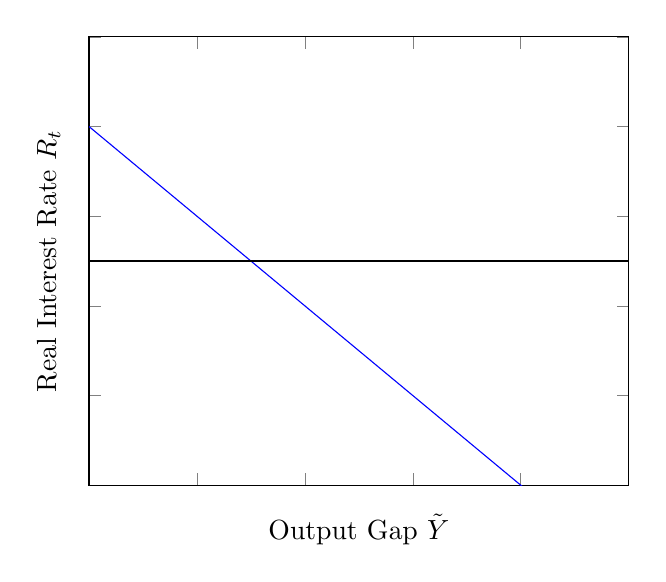
\begin{tikzpicture}
\begin{axis}[xlabel={Output Gap $\og$},ylabel={Real Interest Rate $R_t$},ymin=0,ymax=10,xmin=0,xmax=10,scale=1,yticklabels={,,}, xticklabels={,,}]
\addplot[blue, domain=0:10]
{-x+8};
\addplot[black, domain=0:10]
{5};
\end{axis}
\end{tikzpicture}
\caption{\color{blue}IS-\color{black}MP Diagram}
\end{figure}

\section{Examples of Shocks}

This is how we derive the IS-MP diagram, useful for life and the rest of this course. Let's go over a few examples of shocks to the IS-MP. Simply because we can. You will notice that these are from your Pset. Because I made them muahaha.

Let's suppose that there's a temporary consumption boom that lasts only for one period.

\begin{figure}[H]
\centering
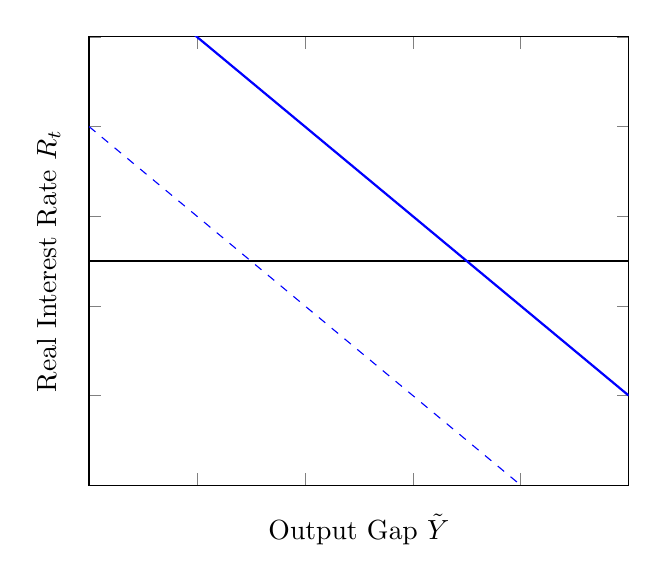
\begin{tikzpicture}
\begin{axis}[xlabel={Output Gap $\og$},ylabel={Real Interest Rate $R_t$},ymin=0,ymax=10,xmin=0,xmax=10,scale=1,yticklabels={,,}, xticklabels={,,}]
\addplot[black, domain=0:10]
{5};
\addplot[blue, domain=0:10, dashed]
{-x+8};
\addplot[blue, domain=0:10, thick]
{-x+12};
\end{axis}
\end{tikzpicture}
\caption{\color{blue}IS-\color{black}MP Diagram}
\end{figure}

This boom means that the IS curve shifts to the right. At the same old nominal interest
rate, this creates a rise in short-run output.

If you were the chair of the Fed, you'd do this.

\begin{figure}[H]
\centering
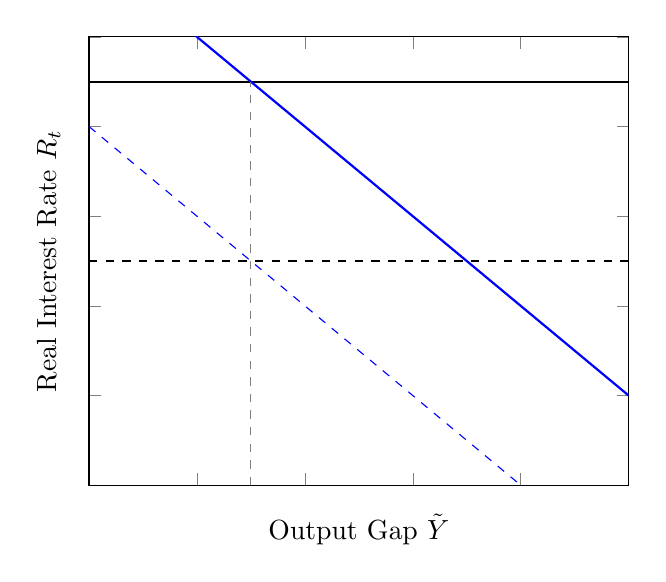
\begin{tikzpicture}
\begin{axis}[xlabel={Output Gap $\og$},ylabel={Real Interest Rate $R_t$},ymin=0,ymax=10,xmin=0,xmax=10,scale=1,yticklabels={,,}, xticklabels={,,}]
\addplot[black, domain=0:10, dashed]
{5};
\addplot[black, domain=0:10, thick]
{9};
\addplot[blue, domain=0:10, dashed]
{-x+8};
\addplot[blue, domain=0:10, thick]
{-x+12};
\addplot[gray, domain=0:10, dashed]
coordinates{(3,0) (3,9)};
\end{axis}
\end{tikzpicture}
\caption{\color{blue}IS-\color{black}MP Diagram}
\end{figure}

A central bank that cared about keeping short-run output right where it was before the consumption boom would immediately raise the nominal interest rate. This would raise the real interest(since inflation expectations don't change in the short run), which would hurt investment purchases. While consumers would probably consume a bit more of GDP ( due to their optimism, presumably), businesses would consume a bit less(due to the Fed's decision to raise the interest rate).

In IS-MP, this means IS shifts right and then MP shifts up just enough so that short-run output is the same as before the consumption boom.

Let's do more practices.

If consumers become pessimistic about the state of the economy and future productivity
growth...

\begin{figure}[H]
\centering
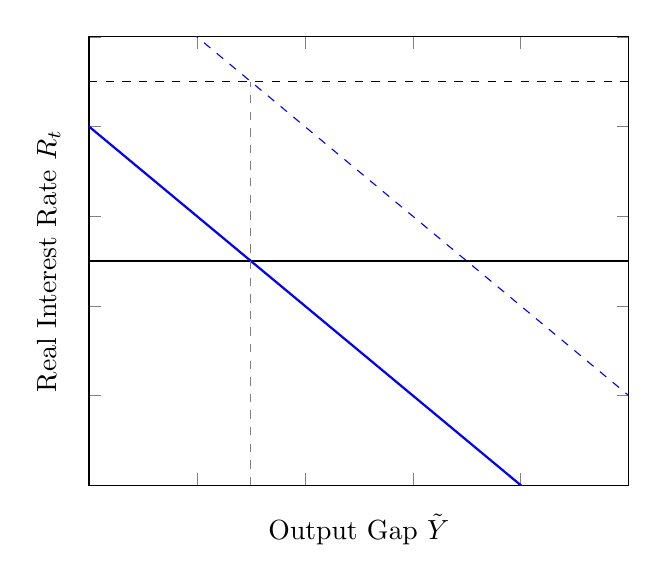
\begin{tikzpicture}
\begin{axis}[xlabel={Output Gap $\og$},ylabel={Real Interest Rate $R_t$},ymin=0,ymax=10,xmin=0,xmax=10,scale=1,yticklabels={,,}, xticklabels={,,}]
\addplot[black, domain=0:10, thick]
{5};
\addplot[black, domain=0:10, dashed]
{9};
\addplot[blue, domain=0:10, thick]
{-x+8};
\addplot[blue, domain=0:10, dashed]
{-x+12};
\addplot[gray, domain=0:10, dashed]
coordinates{(3,0) (3,9)};
\end{axis}
\end{tikzpicture}
\caption{\color{blue}IS-\color{black}MP Diagram}
\end{figure}

This means IS shifts left. Fed should respond by cutting rates(pushing MP down) to put
output gap back to zero.

If there were improvements in productivity and hence marginal product of capital...nothing should change!  An increase in productivity increases potential output only. There are minimal changes in the IS-MP diagram.

If the French suddenly wanted more of our goods, what happens? 

\begin{figure}[H]
\centering
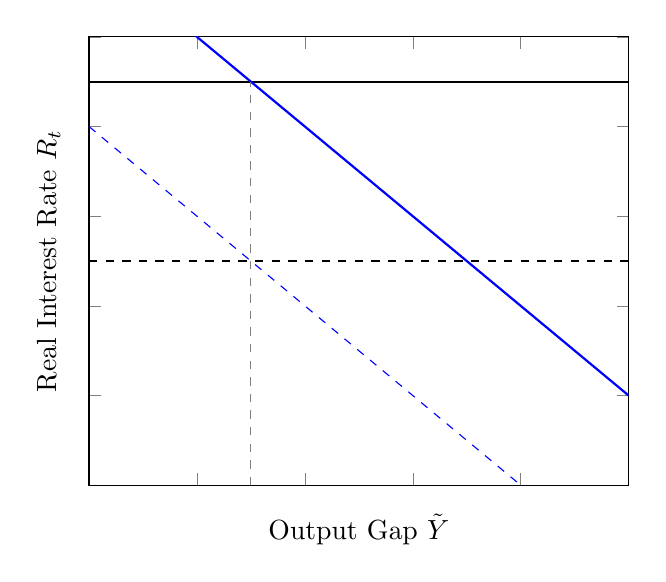
\begin{tikzpicture}
\begin{axis}[xlabel={Output Gap $\og$},ylabel={Real Interest Rate $R_t$},ymin=0,ymax=10,xmin=0,xmax=10,scale=1,yticklabels={,,}, xticklabels={,,}]
\addplot[black, domain=0:10, dashed]
{5};
\addplot[black, domain=0:10, thick]
{9};
\addplot[blue, domain=0:10, dashed]
{-x+8};
\addplot[blue, domain=0:10, thick]
{-x+12};
\addplot[gray, domain=0:10, dashed]
coordinates{(3,0) (3,9)};
\end{axis}
\end{tikzpicture}
\caption{\color{blue}IS-\color{black}MP Diagram}
\end{figure}

IS shifts to the right. Fed should raise MP until output gap is back to zero.

If we suddenly wanted more French goods, what happens?

\begin{figure}[H]
\centering
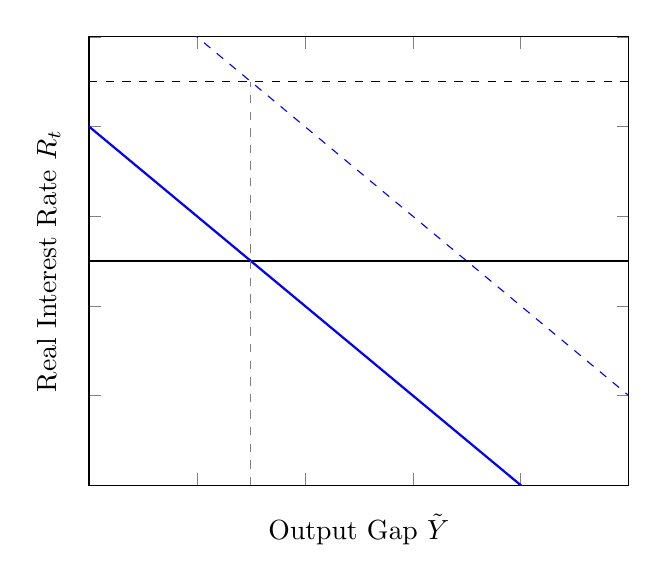
\begin{tikzpicture}
\begin{axis}[xlabel={Output Gap $\og$},ylabel={Real Interest Rate $R_t$},ymin=0,ymax=10,xmin=0,xmax=10,scale=1,yticklabels={,,}, xticklabels={,,}]
\addplot[black, domain=0:10, thick]
{5};
\addplot[black, domain=0:10, dashed]
{9};
\addplot[blue, domain=0:10, thick]
{-x+8};
\addplot[blue, domain=0:10, dashed]
{-x+12};
\addplot[gray, domain=0:10, dashed]
coordinates{(3,0) (3,9)};
\end{axis}
\end{tikzpicture}
\caption{\color{blue}IS-\color{black}MP Diagram}
\end{figure}

IS shifts left. This means fewer consumer goods will be made in the United States. Fed should cut MP until output gap is back to zero

What happens during an earthquake (that destroys only potential output. Everyone is miraculously alive)? Earthquake destroys capital so potential output decreases. There are minimal changes in IS- MP diagram.

\section{What So Far}

So far, we know this.

\begin{itemize}
\item The central bank can set the nominal interest rate
\item With the Fisher equation, the central bank can manipulate the real interest rate
\item With the real interest rate (and the IS curve), the central bank can manipulate the output gap (and unemployment which we can find using Okun's Law)
\item Accordingly, it decides the level of inflation on the Phillips Curve
\end{itemize}

So let's see how we can use this to analyze shocks. We always have two diagrams now:

\begin{figure}[H]
\begin{subfigure}[b]{0.5\textwidth}
\centering
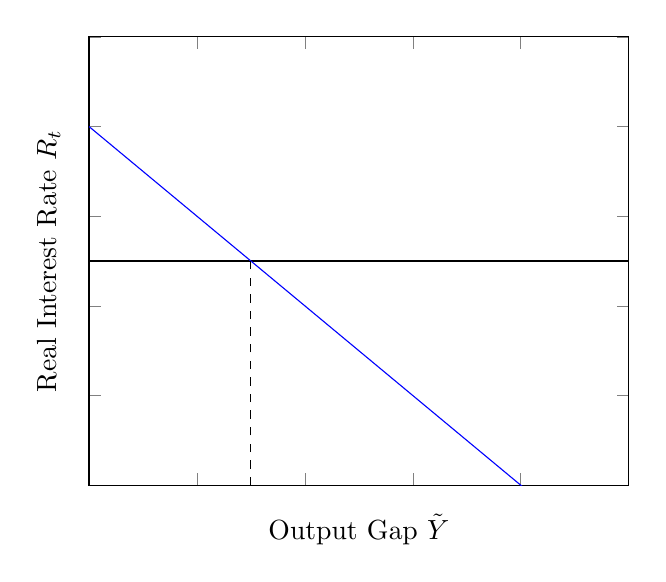
\begin{tikzpicture}
\begin{axis}[xlabel={Output Gap $\og$},ylabel={Real Interest Rate $R_t$},yticklabels={,,}, xticklabels={,,},ymin=0,ymax=10,xmin=0,xmax=10]
\addplot[black, domain=0:10]
{5};
\addplot[blue, domain=0:10]
{-x+8};
\addplot[black, domain=0:10, dashed]
coordinates{(3,0) (3,5)};
\end{axis}
\end{tikzpicture}
\caption{\color{blue}IS-\color{black}MP Diagram}
\end{subfigure}
\hspace{2ex}
\begin{subfigure}[b]{0.5\textwidth}
\centering
\begin{tikzpicture}
\begin{axis}[xlabel={Output Gap $\og$},ylabel={Inflation $\pi_t$},yticklabels={,,}, xticklabels={,,},ymin=0,ymax=10,xmin=0,xmax=10]
\addplot[black, domain=0:10]
{x};
\addplot[black, domain=0:10, dashed]
coordinates{(5,0) (5,5)};
\end{axis}
\end{tikzpicture}
\caption{Phillips Curve}
\end{subfigure}
\caption{Entire Economy}
\end{figure}

Now assume that we were originally at full employment. That's the point indicated by the dotted line.

What if we had an external shock that shifted the IS curve outwards? Then, IS shifts out. And we have a positive output gap. That will be reflected in the Phillips Curve too as we shift to a higher part of the same Phillips curve. That's what happens for this time period.

\begin{figure}[H]
\begin{subfigure}[b]{0.5\textwidth}
\centering
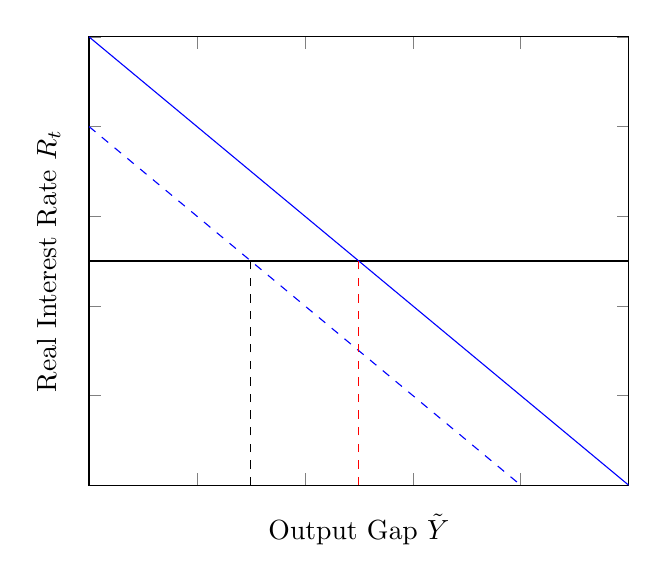
\begin{tikzpicture}
\begin{axis}[xlabel={Output Gap $\og$},ylabel={Real Interest Rate $R_t$},yticklabels={,,}, xticklabels={,,},ymin=0,ymax=10,xmin=0,xmax=10]
\addplot[black, domain=0:10]
{5};
\addplot[blue, domain=0:10, dashed]
{-x+8};
\addplot[blue, domain=0:10]
{-x+10};
\addplot[black, domain=0:10, dashed]
coordinates{(3,0) (3,5)};
\addplot[red, domain=0:10, dashed]
coordinates{(5,0) (5,5)};
\end{axis}
\end{tikzpicture}
\caption{\color{blue}IS-\color{black}MP Diagram}
\end{subfigure}
\hspace{2ex}
\begin{subfigure}[b]{0.5\textwidth}
\centering
\begin{tikzpicture}
\begin{axis}[xlabel={Output Gap $\og$},ylabel={Inflation $\pi_t$},yticklabels={,,}, xticklabels={,,},ymin=0,ymax=10,xmin=0,xmax=10]
\addplot[black, domain=0:10]
{x};
\addplot[black, domain=0:10, dashed]
coordinates{(5,0) (5,5)};
\addplot[red, domain=0:10, dashed]
coordinates{(7,0) (7,7)};
\end{axis}
\end{tikzpicture}
\caption{Phillips Curve}
\end{subfigure}
\caption{Entire Economy}
\end{figure}

Now our Phillips Curve doesn't stay constant in the next period. Nope, it shifts up because people are shmaaaaart. (or adaptive expectations. Professor Phelps please don't kill me for saying this)

\begin{figure}[H]
\begin{subfigure}[b]{0.5\textwidth}
\centering
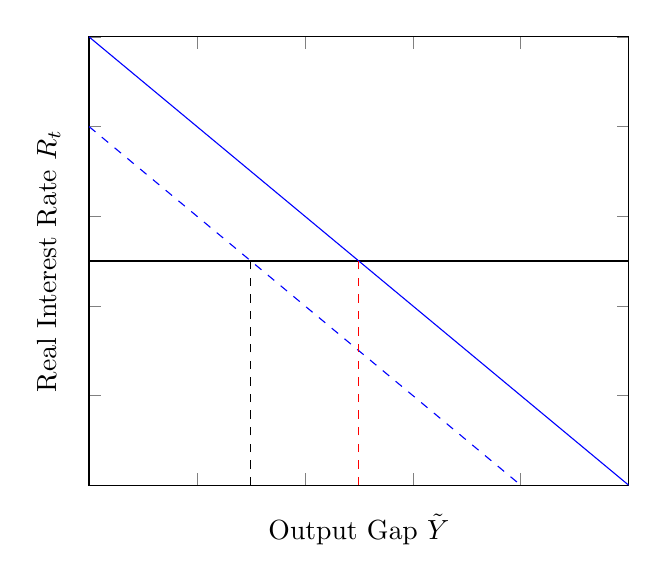
\begin{tikzpicture}
\begin{axis}[xlabel={Output Gap $\og$},ylabel={Real Interest Rate $R_t$},yticklabels={,,}, xticklabels={,,},ymin=0,ymax=10,xmin=0,xmax=10]
\addplot[black, domain=0:10]
{5};
\addplot[blue, domain=0:10, dashed]
{-x+8};
\addplot[blue, domain=0:10]
{-x+10};
\addplot[black, domain=0:10, dashed]
coordinates{(3,0) (3,5)};
\addplot[red, domain=0:10, dashed]
coordinates{(5,0) (5,5)};
\end{axis}
\end{tikzpicture}
\caption{\color{blue}IS-\color{black}MP Diagram}
\end{subfigure}
\hspace{2ex}
\begin{subfigure}[b]{0.5\textwidth}
\centering
\begin{tikzpicture}
\begin{axis}[xlabel={Output Gap $\og$},ylabel={Inflation $\pi_t$},yticklabels={,,}, xticklabels={,,},ymin=0,ymax=10,xmin=0,xmax=10]
\addplot[black, domain=0:10, dashed]
{x};
\addplot[black, domain=0:10]
{x+2};
\addplot[black, domain=0:10, dashed]
coordinates{(5,0) (5,5)};
\addplot[red, domain=0:10, dashed]
coordinates{(7,0) (7,9)};
\end{axis}
\end{tikzpicture}
\caption{Phillips Curve}
\end{subfigure}
\caption{Entire Economy}
\end{figure}

Now the central bank sees this and isn't happy. The inflation is gonna spiral out of control. So, it raises nominal interest rates, which increases real interest rates such that output gap goes back to the full employment level.

\begin{figure}[H]
\begin{subfigure}[b]{0.5\textwidth}
\centering
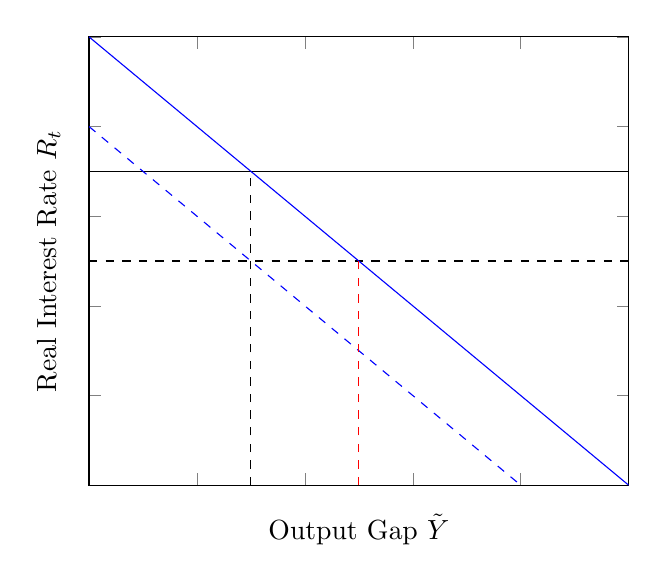
\begin{tikzpicture}
\begin{axis}[xlabel={Output Gap $\og$},ylabel={Real Interest Rate $R_t$},yticklabels={,,}, xticklabels={,,},ymin=0,ymax=10,xmin=0,xmax=10]
\addplot[black, domain=0:10, dashed]
{5};
\addplot[black, domain=0:10]
{7};
\addplot[blue, domain=0:10, dashed]
{-x+8};
\addplot[blue, domain=0:10]
{-x+10};
\addplot[black, domain=0:10, dashed]
coordinates{(3,0) (3,7)};
\addplot[red, domain=0:10, dashed]
coordinates{(5,0) (5,5)};
\end{axis}
\end{tikzpicture}
\caption{\color{blue}IS-\color{black}MP Diagram}
\end{subfigure}
\hspace{2ex}
\begin{subfigure}[b]{0.5\textwidth}
\centering
\begin{tikzpicture}
\begin{axis}[xlabel={Output Gap $\og$},ylabel={Inflation $\pi_t$},yticklabels={,,}, xticklabels={,,},ymin=0,ymax=10,xmin=0,xmax=10]
\addplot[black, domain=0:10, dashed]
{x};
\addplot[black, domain=0:10]
{x+2};
\addplot[black, domain=0:10, dashed]
coordinates{(5,0) (5,7)};
\addplot[red, domain=0:10, dashed]
coordinates{(7,0) (7,9)};
\end{axis}
\end{tikzpicture}
\caption{Phillips Curve}
\end{subfigure}
\caption{Entire Economy}
\end{figure}

Then, we first get zero output gap from our IS-MP diagram with a resulting higher real interest rate. Since we're at zero output gap, inflation stops spiraling out of control. We stay with a permanently higher inflation level. 

You can work out the equations for these. It's quite a handful, but it's not difficult at all.

\section{Formalizing The Central Bank's Actions}

So far, we think that the central bank kind of sets the MP curve using a vague set of rules. Sometimes, it aims to achieve zero output gap. Otherwise, it aims to control inflation.

Let's come up with an "ideal" central bank that aims to do one thing and one thing only: \textbf{control inflation}. Then, it will change real interest rates whenever inflation is away from its "target" level. Hence, it controls real interest rate such that

\[R_t - \bar{r} = \bar{m} (\pi_t - \bar{\pi_t}) \]

where $R_t$ is the real interest rate, $\bar{r}$ is the "natural" interest rate (you can think of it as long run interest rate), $\bar{m}$ is how aggressive the government is with monetary policy, $\pi_t$ being inflation and $\bar{\pi_t}$ being the inflation target.

\section{Aggregate Demand and Supply}

Then let's see what we have now

\begin{enumerate}
\item Monetary Policy: $R_t - \bar{r} = \bar{m} (\pi_t - \bar{\pi})$
\item Investment Saving: $\og_t = \bar{a}_t - \bar{b} (R_t - \bar{r})$
\item Phillips Curve: $\pi_t = \pi_{t-1} + \bar{v} \og_t + \bar{o}_t$ 
\item Okun's Law: $\og_t = -2 (u_t - \bar{u})$
\end{enumerate}

We can assume that the IS-MP will always be equilibrium. When we take that assumption, we can equate those two and come up with an \textbf{Aggregate Demand}

\[\og_t = \bar{a}_t - \bar{b} \bar{m} (\pi_t - \bar{\pi} ) \]

Our Phillips Curve acts as the \textbf{Aggregate Supply}

So together,

\begin{align*}
\og_t &= \bar{a}_t - \bar{b} \bar{m} (\pi_t - \bar{\pi} ) \\
\pi_t &= \pi_{t-1} + \bar{v} \og_t + \bar{o}_t
\end{align*}

Plot them with $\pi_t$ on the y-axis and $\og_t$ on the x-axis and we get

\begin{figure}[H]
\centering
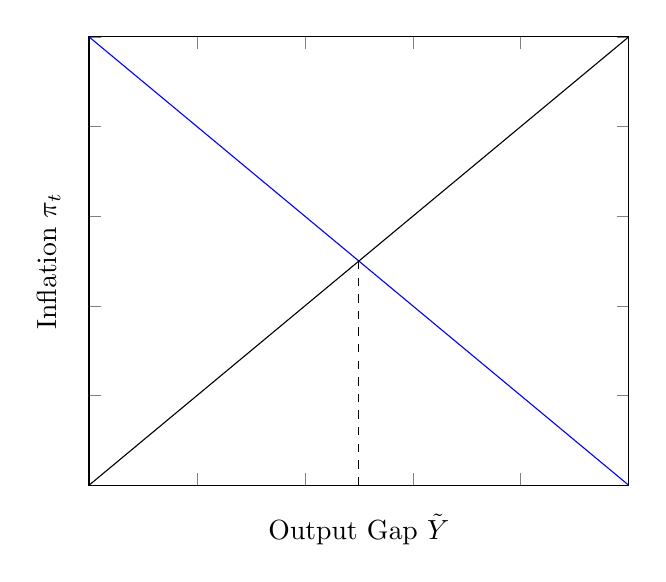
\begin{tikzpicture}
\begin{axis}[xlabel={Output Gap $\og$},ylabel={Inflation $\pi_t$},ymin=0,ymax=10,xmin=0,xmax=10,scale=1,yticklabels={,,}, xticklabels={,,}]
\addplot[blue, domain=0:10]
{-x+10};
\addplot[black, domain=0:10]
{x};
\addplot[black, domain=0:10,dashed]
coordinates{(5,0) (5,5)};
\end{axis}
\end{tikzpicture}
\caption{\color{blue}AD \color{black} AS Diagram}
\end{figure}

The dashed line indicates the full employment level, hence where $\og_t = 0$. This diagram captures the whole model in one single figure. How so?

Let's suppose that an external shock moves the IS curve to the right. It's the exact same exercise as we did earlier, just that we're combining everything on one diagram.

\begin{figure}[H]
\centering
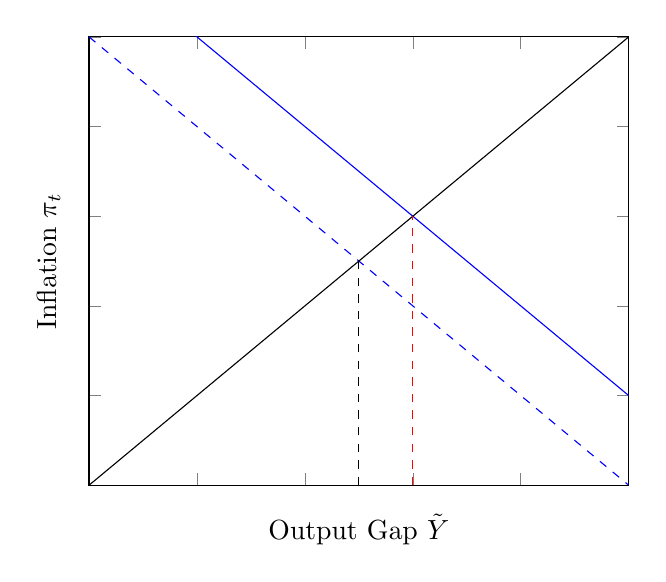
\begin{tikzpicture}
\begin{axis}[xlabel={Output Gap $\og$},ylabel={Inflation $\pi_t$},ymin=0,ymax=10,xmin=0,xmax=10,scale=1,yticklabels={,,}, xticklabels={,,}]
\addplot[blue, domain=0:10, dashed]
{-x+10};
\addplot[blue, domain=0:10]
{-x+12};
\addplot[black, domain=0:10]
{x};
\addplot[black, domain=0:10,dashed]
coordinates{(5,0) (5,5)};
\addplot[red, domain=0:10,dashed]
coordinates{(6,0) (6,6)};
\end{axis}
\end{tikzpicture}
\caption{\color{blue}AD \color{black} AS Diagram}
\end{figure}

Now with a higher IS due to the shock, we arrive at a higher point on our Phillips Curve.

During the next time period, our Phillips Curve (or the AS) shifts up due to them smarties.

\begin{figure}[H]
\centering
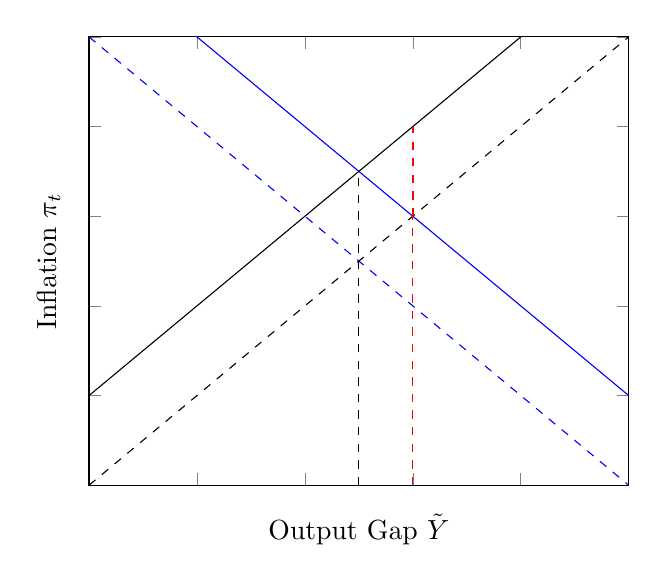
\begin{tikzpicture}
\begin{axis}[xlabel={Output Gap $\og$},ylabel={Inflation $\pi_t$},ymin=0,ymax=10,xmin=0,xmax=10,scale=1,yticklabels={,,}, xticklabels={,,}]
\addplot[blue, domain=0:10, dashed]
{-x+10};
\addplot[blue, domain=0:10]
{-x+12};
\addplot[black, domain=0:10, dashed]
{x};
\addplot[black, domain=0:10]
{x+2};
\addplot[black, domain=0:10,dashed]
coordinates{(5,0) (5,7)};
\addplot[red, domain=0:10,dashed]
coordinates{(6,0) (6,6)};
\addplot[red, domain=0:10,dashed,thick]
coordinates{(6,6) (6,8)};
\end{axis}
\end{tikzpicture}
\caption{\color{blue}AD \color{black} AS Diagram}
\end{figure}

Now the funny thing is as it moves up, we move back to the original output gap. How does that happen? Well remember in our original analysis, we said that the Phillips Curve shifts up, and the central bank shifts up the monetary policy curve to make output gap go back to the original level in response to increasing inflations? Well, we've simply combined this effect. Note that it is due to the effect of the central bank that inflation did not increase by the full extent of the upward shift of the Phillips Curve (as indicated by the thick red line).  

We end up with a permanently higher inflation level and the original output gap, same as our previous analysis. Same shit, just a lot more convenient.







\end{document}